\documentclass[times, twoside, watermark]{zHenriquesLab-StyleBioRxiv}
\usepackage{blindtext}

% Please give the surname of the lead author for the running footer


\begin{document}

\title{The Black Box Nature of AI, Ethical and Philosophical Implications}

% Use letters for affiliations, numbers to show equal authorship (if applicable) and to indicate the corresponding author
\author[1,\Letter]{Sara Borello, Keita Jacopo Viganò}

\affil[1]{Msc Students Data Science Unimib}

\maketitle

%TC:break Abstract
%the command above serves to have a word count for the abstract
\begin{abstract}
Our research aims to explore the issues that come from using AI technologies that are not transparent. We look closely at the idea of making AI models clearer and easier to understand, especially using the human-centered approach proposed by Capone and Bertolaso. We will examine the ethical and philosophical problems that arise because these technologies are not open and accountable and how thinking about these issues from a philosophical point of view can help improve how AI systems interact with people, building trust and understanding while tackling the shortcomings of current approaches that focus just on technical solutions and transparency.
\end {abstract}

\section*{Introduction}

The advent of the Fourth Industrial Revolution has solidified artificial intelligence as a constant presence in our daily lives. The global AI landscape has experienced significant growth in recent years, with notable increases in both investments and market valuations. In 2023, the global AI market was valued at approximately \$196.63 billion and is projected to expand at a compound annual growth rate (CAGR) of 36.6\% from 2024 to 2030, reaching an estimated \$826.70 billion by 2030 \cite{ai_market}. Private investment has been a major driver of this growth. In 2023, the United States led the world with \$ 62.5 billion in private AI investments, followed by China with \$ 7.3 billion. The European Union and the United Kingdom together attracted \$ 9 billion in private AI investments during the same period \cite{ai_regulations}. These figures underscore the growing significance of technologies such as machine learning and Large Language Models, which power innovative tools in diverse fields, ranging from marketing to medical diagnostics, and autonomous driving. For example, GitHub Copilot uses OpenAI Codex (a variant of GPT) to provide real-time code suggestions and auto-completions in popular IDEs \cite{github_copilot}. Meanwhile, Morgan Stanley has integrated OpenAI’s GPT-4 to organize and analyze its extensive knowledge base of over 16,000 financial advisors, enabling rapid retrieval of research, policies, and analyst insights through an LLM-powered system \cite{openai_morgan_stanley}.

However, despite their impressive capabilities, these models are often regarded as \textit{``black boxes,''} a term that denotes the lack of transparency in understanding their internal decision-making processes. While black-box models excel in predictive power, their opacity raises critical ethical and operational concerns \cite{hassija2024xai}. In sensitive domains such as medicine, relying on systems whose decision-making processes are inscrutable can be perilous, as any diagnostic or therapeutic recommendation generated by an LLM must be accompanied by comprehensible justifications for medical professionals and patients alike to build trust, ensure acceptance, and enable continuous improvement.

The concept of explainability varies significantly across different contexts and applications worldwide \cite{typeexplain}:

\begin{itemize}
    \item \textbf{Justification of Critical Decisions}: Transparent systems are necessary to comply with regulations, such as the \textit{``right to explanation''} enshrined in the GDPR. This is particularly vital in areas where decisions have profound consequences, including healthcare, finance, and criminal justice.
    \item \textbf{Model Accountability and Debugging}: Explainability aids in identifying vulnerabilities and rectifying errors in AI systems promptly. For example, understanding an LLM’s reasoning could uncover biases or inaccuracies in its training data, leading to targeted improvements.
    \item \textbf{Facilitation of Iterative Improvements}: A deeper understanding of AI mechanisms enhances their refinement. Explainable models allow developers and researchers to iteratively enhance performance based on clear insights rather than trial-and-error approaches.
\end{itemize}


\section*{ML Modes and XAI}
Traditional machine learning models, such as linear regression and decision trees, are often celebrated for their simplicity and interpretability. Their straightforward structures, characterized by a limited number of parameters, create a clear relationship between input variables and predictions. This enables users to understand the underlying decision-making mechanisms with relative ease, fostering trust and transparency \cite{james2013introduction}.

Explainable AI (XAI) takes this concept further by addressing the interpretability challenges posed by more complex models, such as neural networks and ensemble methods \cite{typeexplain}. While traditional models inherently provide tools for understanding, such as coefficients in linear regression or feature importance metrics in decision trees, XAI aims to generalize interpretability across all model types, regardless of their complexity. Advanced methods like SHAP \cite{lundberg2017unified} and LIME \cite{ribeiro2016should} bridge the gap by offering model-agnostic techniques that provide both local explanations (clarifying individual predictions) and global insights (revealing overarching model behavior). These approaches enable practitioners to quantify the contribution of each feature, visualize decision boundaries, and even assess model fairness, making opaque models more accessible and transparent.

%Just for kicks here's a citation \cite{ai_regulations}. And a reference to a supplement \cref{note:Note1}. And \nameref{note:Note1}.%



\section*{Critique of XAI}
Traditional XAI methods like SHAP and LIME, despite their precision and mathematical rigor, often fail to meet the practical needs of non-expert users, particularly in critical domains such as healthcare and finance. Although these techniques provide precise, mathematically rigorous explanations, they fail to translate these insights into forms that are easily understandable and actionable for practitioners without technical expertise \cite{vernaza2023contextualising}. For instance, a medical professional interpreting SHAP values may struggle to contextualize the quantified contributions of variables like biomarkers within a broader diagnostic framework, rendering the explanation insufficiently actionable. Similarly, financial analysts may find LIME's feature attributions too abstract to make confident decisions in dynamic market environments.
Some challenges of XAI reported by Hans de Bruijn et al. \cite{DEBRUIJN2022101666} are illustrated in Figure~\ref{fig:challanges}.

\begin{figure}[H]
\centering
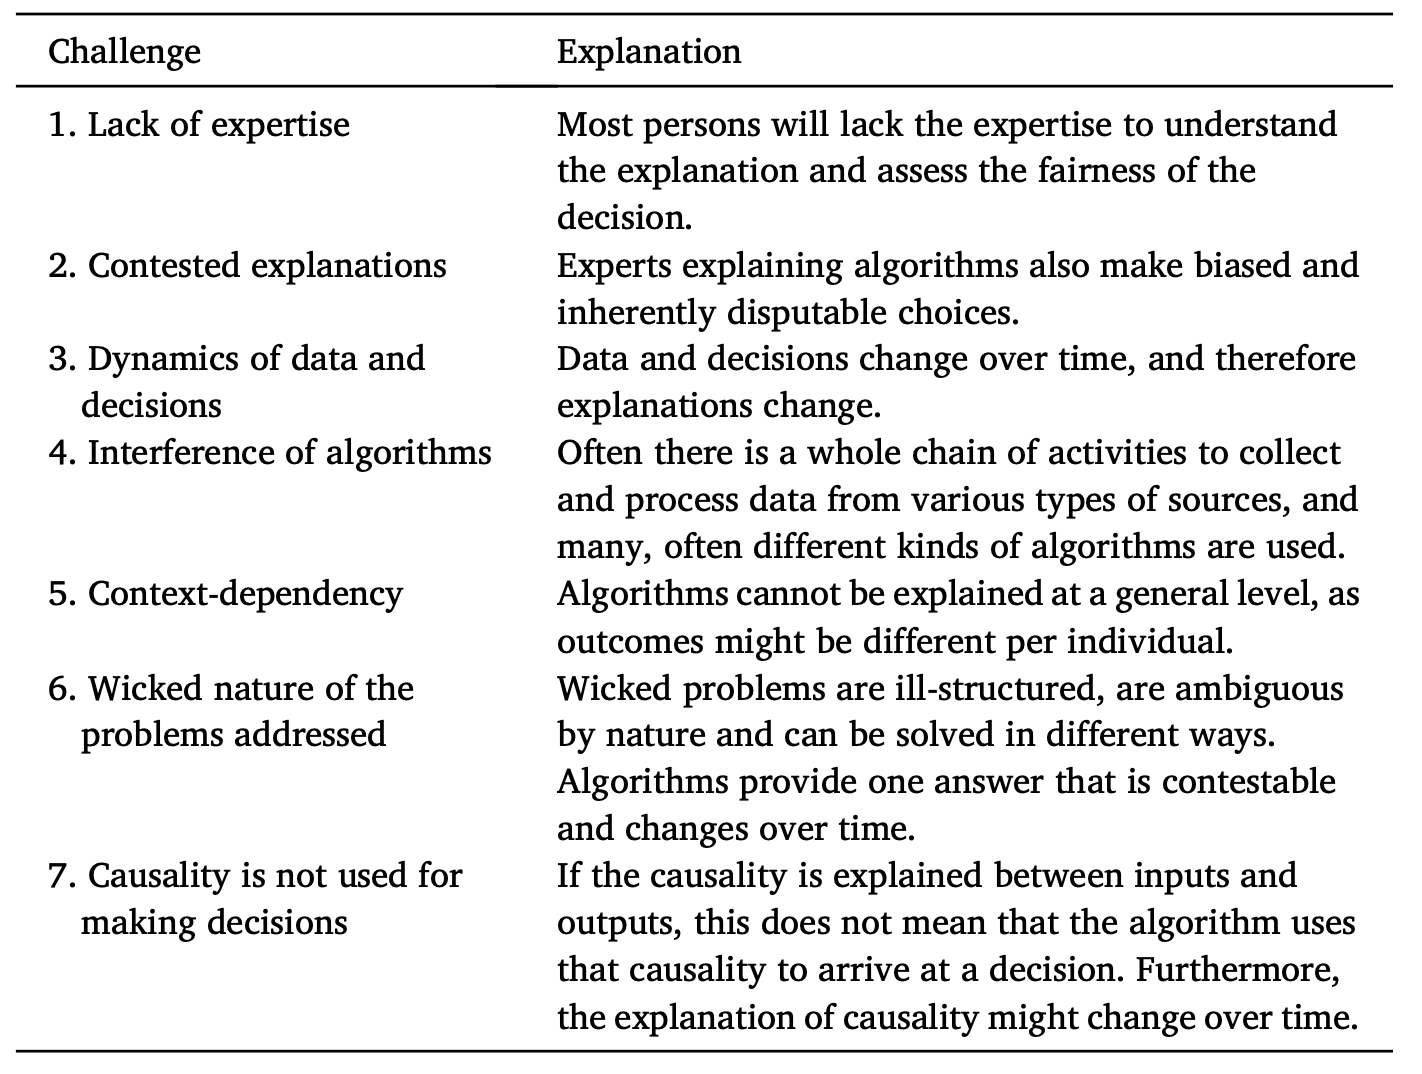
\includegraphics[width=.8\linewidth]{Figures/challangesXAI.png}
\caption{Challenges of XAI as reported by Hans de Bruijn et al. \cite{DEBRUIJN2022101666}.}
\label{fig:challanges}
\end{figure}


While XAI has made strides in explaining traditional ML models, the advent of LLMs has reintroduced the interpretability challenge. 

LLMs, such as BERT \cite{devlin2018bert} and GPT \cite{radford2019language}, leverage the Transformer architecture to operate in high-dimensional spaces with billions of parameters. These models capture complex interactions within the input data and exhibit emergent abilities that are not explicitly programmed. However, this architectural complexity obscures their inner workings, making it challenging to interpret and explain their predictions \cite{vaswani2017attention}.

Unlike traditional ML models, where explanations rely on direct and interpretable mappings between input features and outputs, LLMs encode knowledge across billions of parameters in dense, high-dimensional spaces \cite{devlin2018bert}. This distributed representation makes it difficult to isolate specific contributions or causal pathways leading to a prediction. Attention mechanisms, often used for interpretability, have been shown to lack alignment with true causal importance, offering only partial insights \cite{jain2019attention}. Similarly, probing tasks reveal properties encoded in LLMs but fail to clarify how these are utilized during inference \cite{conneau2018you}. The deeply entangled and non-linear interactions in LLMs further complicate efforts to trace decision-making processes. As a result, traditional XAI approaches fall short, unable to unpack the complexity and opaqueness inherent in LLM architectures, necessitating new paradigms for interpretability.

Emerging methods for improving the explainability of LLMs include innovative approaches like AlphaProof and sparse autoencoders (SAE) \cite{ng2011sparse}. AlphaProof integrates a pre-trained language model with the AlphaZero reinforcement learning algorithm to prove mathematical statements in the formal Lean language, enhancing reasoning through a feedback loop \cite{deepmind2024imo}. By translating natural language problems into formal statements, AlphaProof generates and verifies proof candidates, reinforcing the model's ability to solve increasingly complex problems. SAEs identify active latent variables, linking neural activations to meaningful symbolic concepts, and facilitate mapping neural responses to symbolic structures while addressing the challenge of translating natural language into symbolic representations \cite{elhage2022monosemanticity}. Complementing these methods, Gemma Scope offers token-level hierarchical explanations, improving interpretability in LLMs \cite{deepmind2024gemma}.
These models are still a subject of ongoing research and are not yet widely adopted in business contexts. However, future developments could focus on making them more user-friendly and aligning them with a human-centric approach, which would facilitate their integration into practical applications and everyday workflows.

\section*{Philosophy and Epistemology in Human-Centered Explainability}
The integration of the philosophy of language and epistemology into the framework of Explainable AI offers a transformative avenue for fostering a deeply human-centered approach to the design and deployment of intelligent systems. Drawing on the philosophical insights of Ludwig Wittgenstein, particularly his exploration of the limits of language and the social nature of meaning, this perspective challenges the reductionist notion that explanations are mere computational outputs. Instead, it frames explanations as inherently communicative acts, requiring contextual awareness, shared understanding, and alignment with the cognitive capacities of the audience. Wittgenstein’s proposition that meaning arises through use underscores the importance of tailoring explanations not as static artifacts but as dynamic, interactive processes that evolve through engagement with the user \cite{wittgenstein1953philosophical}.

Epistemology further enriches this framework by highlighting the conditions under which knowledge is acquired, justified, and understood. In particular, the works of Alvin Goldman on epistemic justification \cite{goldman1986epistemology} and Miranda Fricker’s concept of epistemic injustice \cite{fricker2007epistemic}
reveal critical dimensions of explanation that are often overlooked in purely technical models of XAI. By recognizing that users approach AI systems with varying degrees of epistemic authority and cognitive frameworks, a human-centered XAI system must do more than present transparent data; it must actively facilitate understanding. This entails crafting explanations that respect the user's epistemic position, bridging gaps in knowledge, and fostering a sense of cognitive empowerment rather than alienation.

From this perspective, explanations in XAI are not unidirectional or universally interpretable but are better understood as dialogical constructs, co-created through iterative feedback and adaptation to user-specific needs. This dialogical model aligns with philosophical hermeneutics, particularly the work of Hans-Georg Gadamer, who emphasized the fusion of horizons between interlocutors as a prerequisite for genuine understanding \cite{gadamer1975truth}. Similarly, explanations in XAI must engage with the user’s interpretive horizon, respecting their unique background while inviting them into a shared epistemic space where the system’s logic and decision-making processes become comprehensible and relatable.

This approach also challenges the prevailing emphasis on technical transparency as the primary measure of explainability. While transparency is crucial, it is insufficient if it fails to account for the user's ability to meaningfully engage with and interpret the information provided. A human-centered XAI framework shifts the focus toward intelligibility and relational trust, recognizing that understanding is as much a social and psychological phenomenon as it is a technical one. Trust in AI systems is not merely a function of their correctness or reliability but also of their ability to communicate their processes in a way that resonates with the human capacity for understanding, empathy, and ethical reflection.

By embedding these philosophical principles into the design of XAI, we can reimagine AI systems not as opaque oracles but as collaborative partners in the human pursuit of knowledge. These systems, designed with a sensitivity to linguistic, epistemic, and contextual factors, can facilitate not only the effective transfer of information but also the cultivation of deeper insights, ethical awareness, and critical engagement. 

\section*{Neuro-Symbolic Loop in Autonomous Driving}
The neuro-symbolic loop \cite{poterti2024neurosymbolic}, illustrated in Figure~\ref{fig:nesy} and applied in autonomous driving, represents a pioneering integration of neural networks and symbolic reasoning. This approach enhances transparency, reliability, and alignment with human cognition, while embedding a philosophical commitment to reasoning and fostering trust.
 The cycle functions by combining the strengths of neural networks, which process raw inputs like sensor data into symbolic representations, "Pedestrian detected, crossing 5 meters ahead", and symbolic modules, which apply logical rules for decision-making, such as stopping to prevent a collision. This process operates iteratively: It begins with perception and action, continues with post-decision analysis, and culminates in refinement, where logged sensor data and neural activations are revisited using LLMs to extract symbolic concepts and generate human-readable explanations. These explanations not only reveal potential inconsistencies but also refine reasoning, ensuring the system improves with each iteration. Philosophically, this framework resonates with epistemological principles by prioritizing transparency as interpretability and justifiability rather than mere technical clarity. Inspired by Gadamer's "fusion of horizons," it emphasizes understanding as a shared process between human and machine, cultivating trust through the system's ability to reason, learn, and communicate in ways aligned with human cognitive and moral expectations. For instance, if an error occurs—such as a misclassification of a shadow as a pedestrian leading to unnecessary braking—the system transparently reconstructs its logic, offering explanations like, "The vehicle misclassified a shadow as a pedestrian, leading to a false positive stop." This iterative feedback boosts safety and decision-making performance but also establishes the autonomous system as a collaborative and accountable entity, advancing a vision of human-centered autonomy where technology supports humanity with clarity, adaptability, and respect for the intricacies of reasoning and understanding.
\begin{figure}[H]
\centering
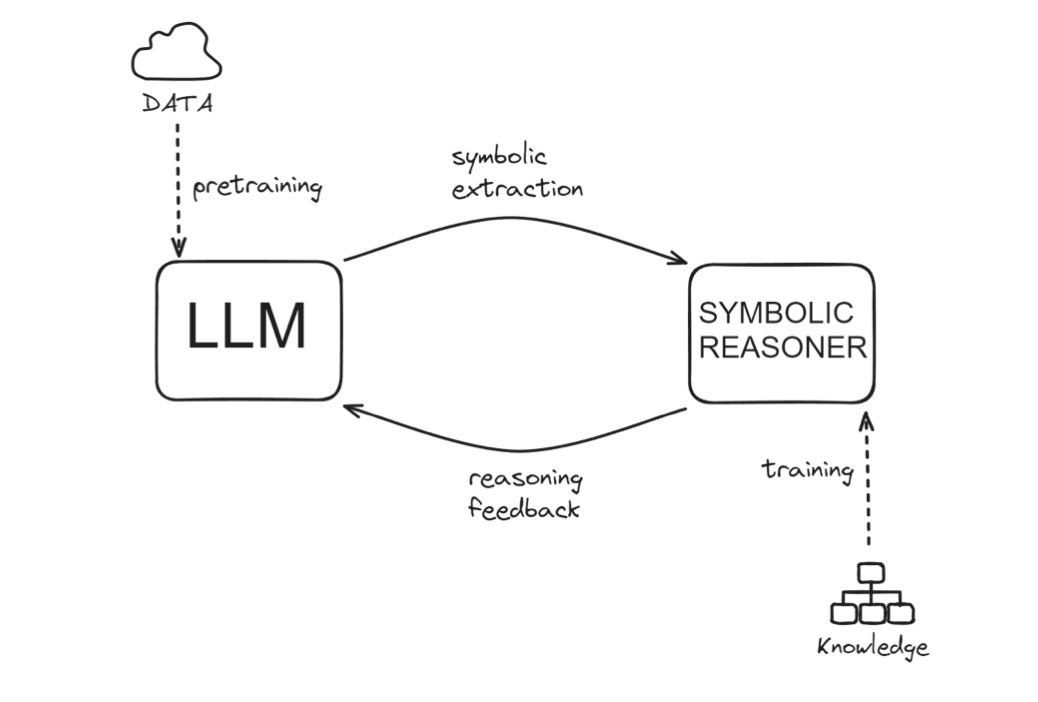
\includegraphics[width=.8\linewidth]{Figures/nesy loop.png}
\caption{NeSy Loop reported by Daniele Potertì \cite{poterti2024neurosymbolic}.}
\label{fig:nesy}
\end{figure}










\section*{Bibliography}
\bibliography{zHenriquesLab-Mendeley}

\end{document}